\documentclass[../../main.tex]{subfiles}

\graphicspath{{images/Projektmanagement/}{../../images/Projektmanagement/}{include_pdf/}{../../include_pdf/}}

\begin{document}
Dieses Kaptitel beschreibt das Projektmanagement des Team 28. Es wird auf die Organisation im Team, die Aufteilung der Arbeitspakete und Zeitplanung eingegangen.

\subsection{Organigramm}
Die Abbildung \ref{fig:organigramm} zeigt die Organisation im Team auf. Das Team ist in die einzelnen Disziplinen Maschinentechnik, Elektrotechnik und Informatik aufgeteilt. Zusätzlich gibt es einen Projektleiter, dieser ist verantwortlich für die Kommunikation mit den Fachdozenten und ist bei allfälligen Abwesenheiten von Teammitgliedern informiert.


\begin{figure}[H] \centering
    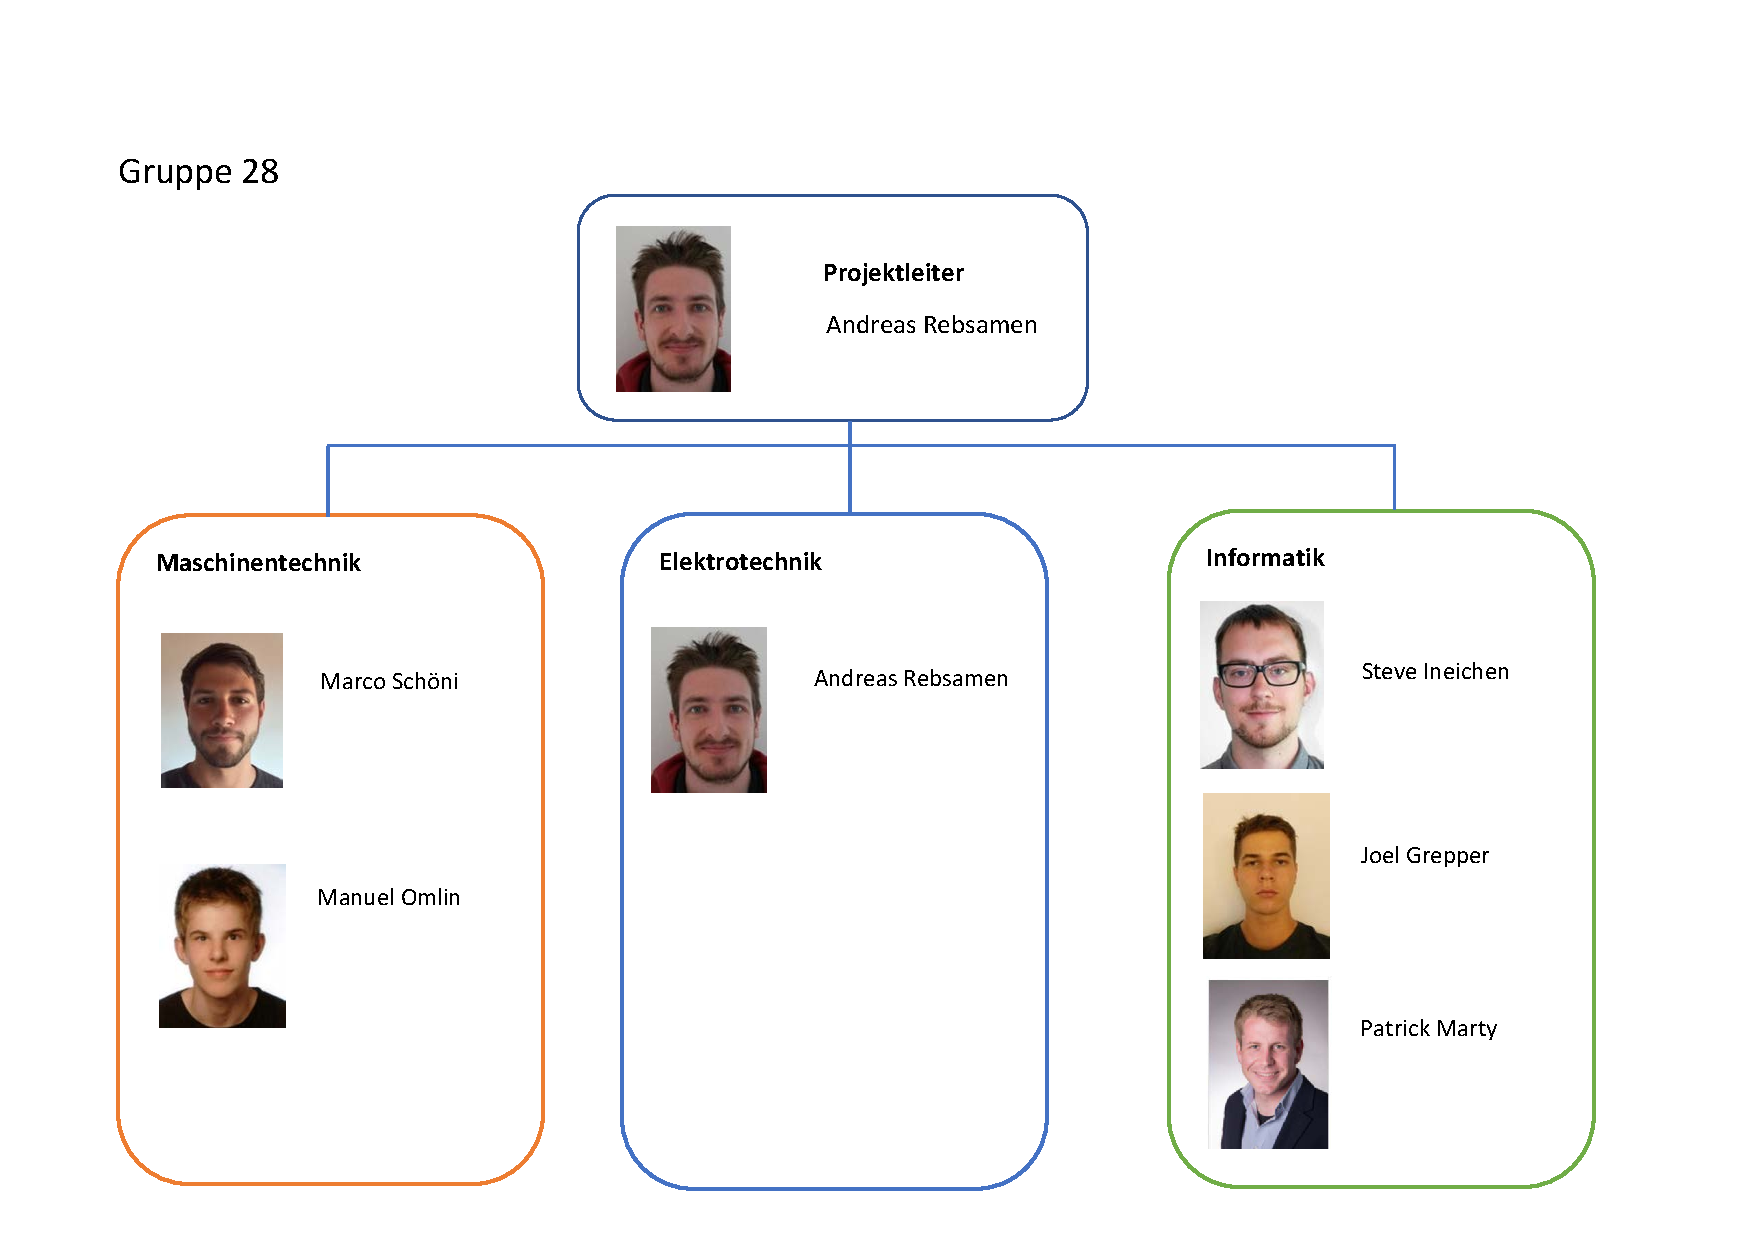
\includegraphics[page=1,width=.9\textwidth, trim=1cm .5cm 1cm 3.2cm, clip]{Organigramm.pdf}
    %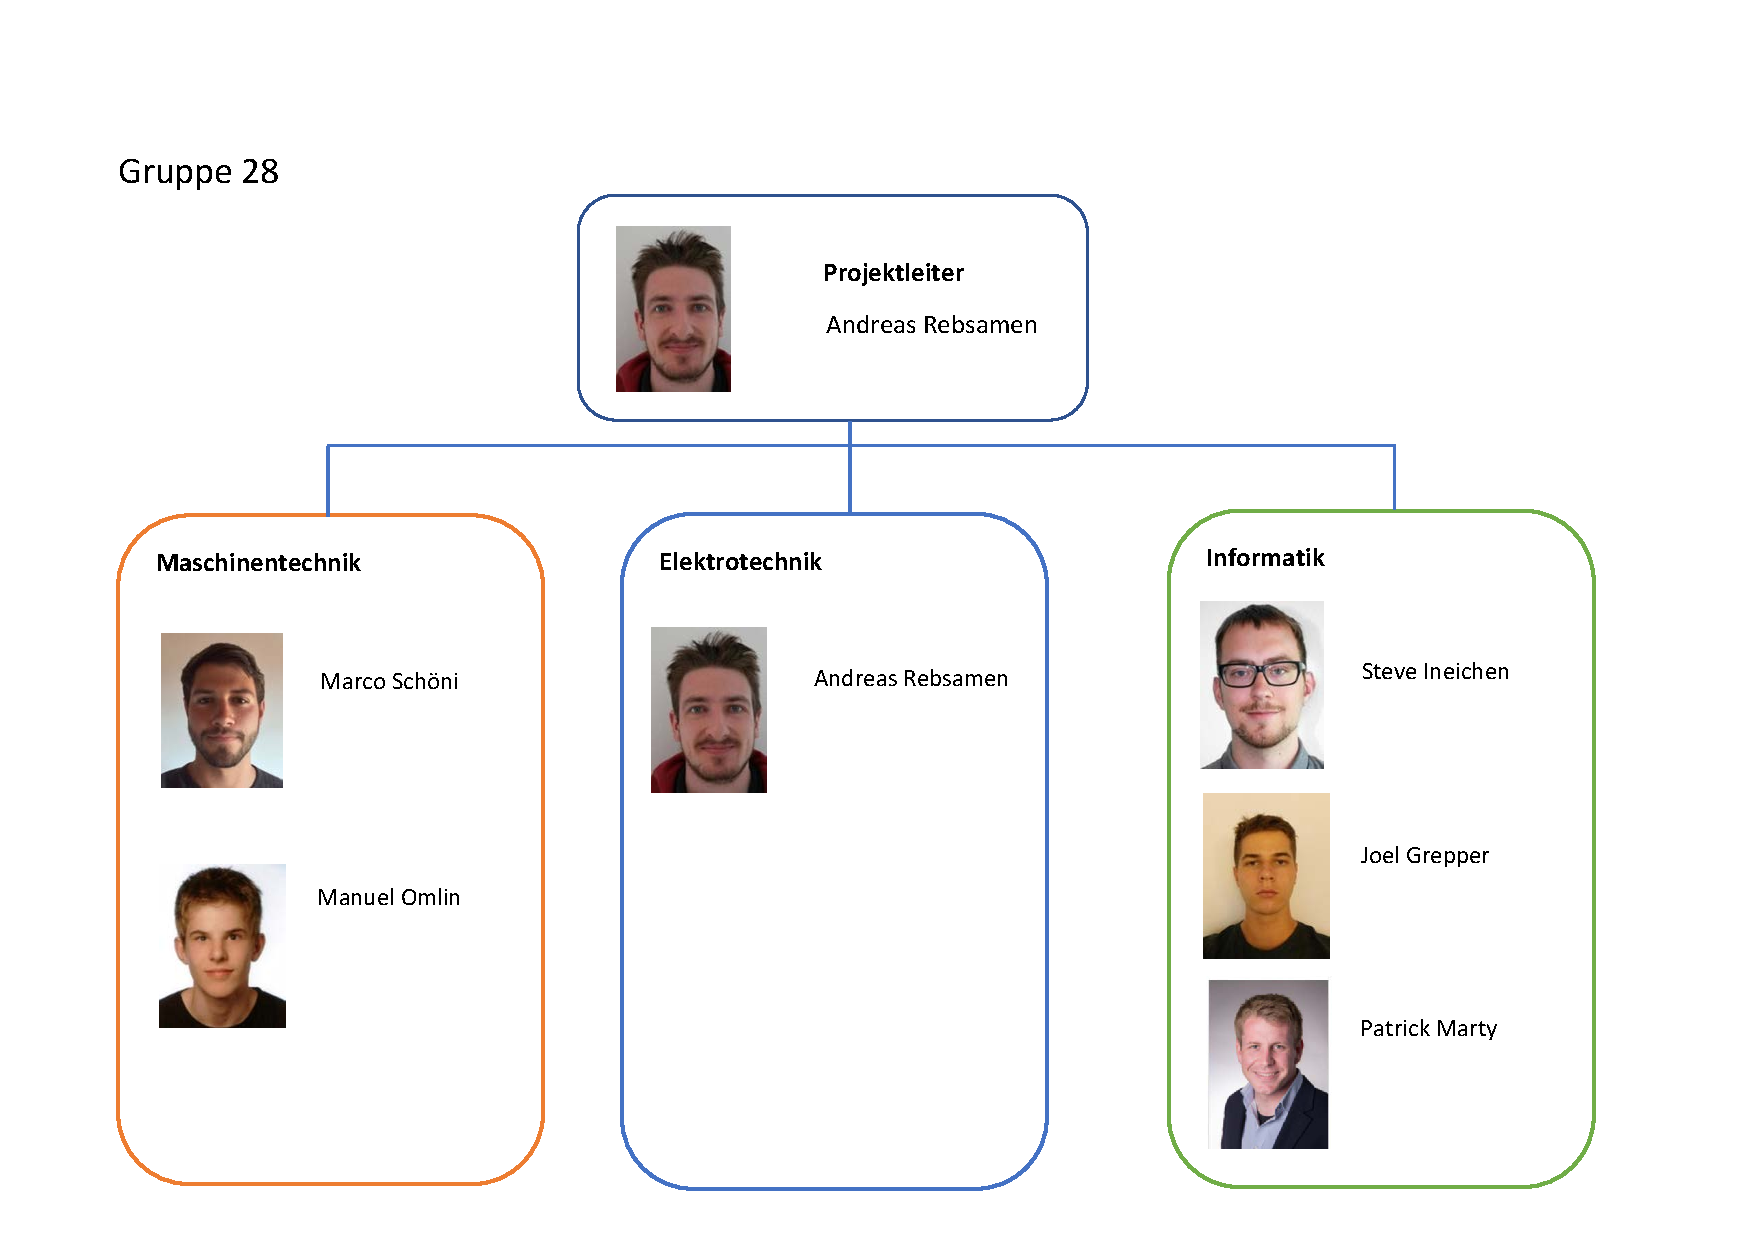
\includepdf[scale=0.8,clip,trim=20mm 7mm 20mm 32mm,pages=-,pagecommand={},nup=1x1, offset=0 -0cm]{Organigramm.pdf}
    \caption{Organigramm Team 28}
    \label{fig:organigramm}
\end{figure}
\pagebreak
\subsection{Zeitplanung}
Mit den groben Arbeitspaketen wurde eine zeitorientierte Projektstruktur (Abbildung \ref{fig:projektplanung}) erstellt. In dieser ist festgehalten, welcher Person oder Disziplin ein Arbeitspaket zugeteilt ist, ob diese neu, in Arbeit oder abgeschlossen ist. \\

\begin{figure}[H] \centering
    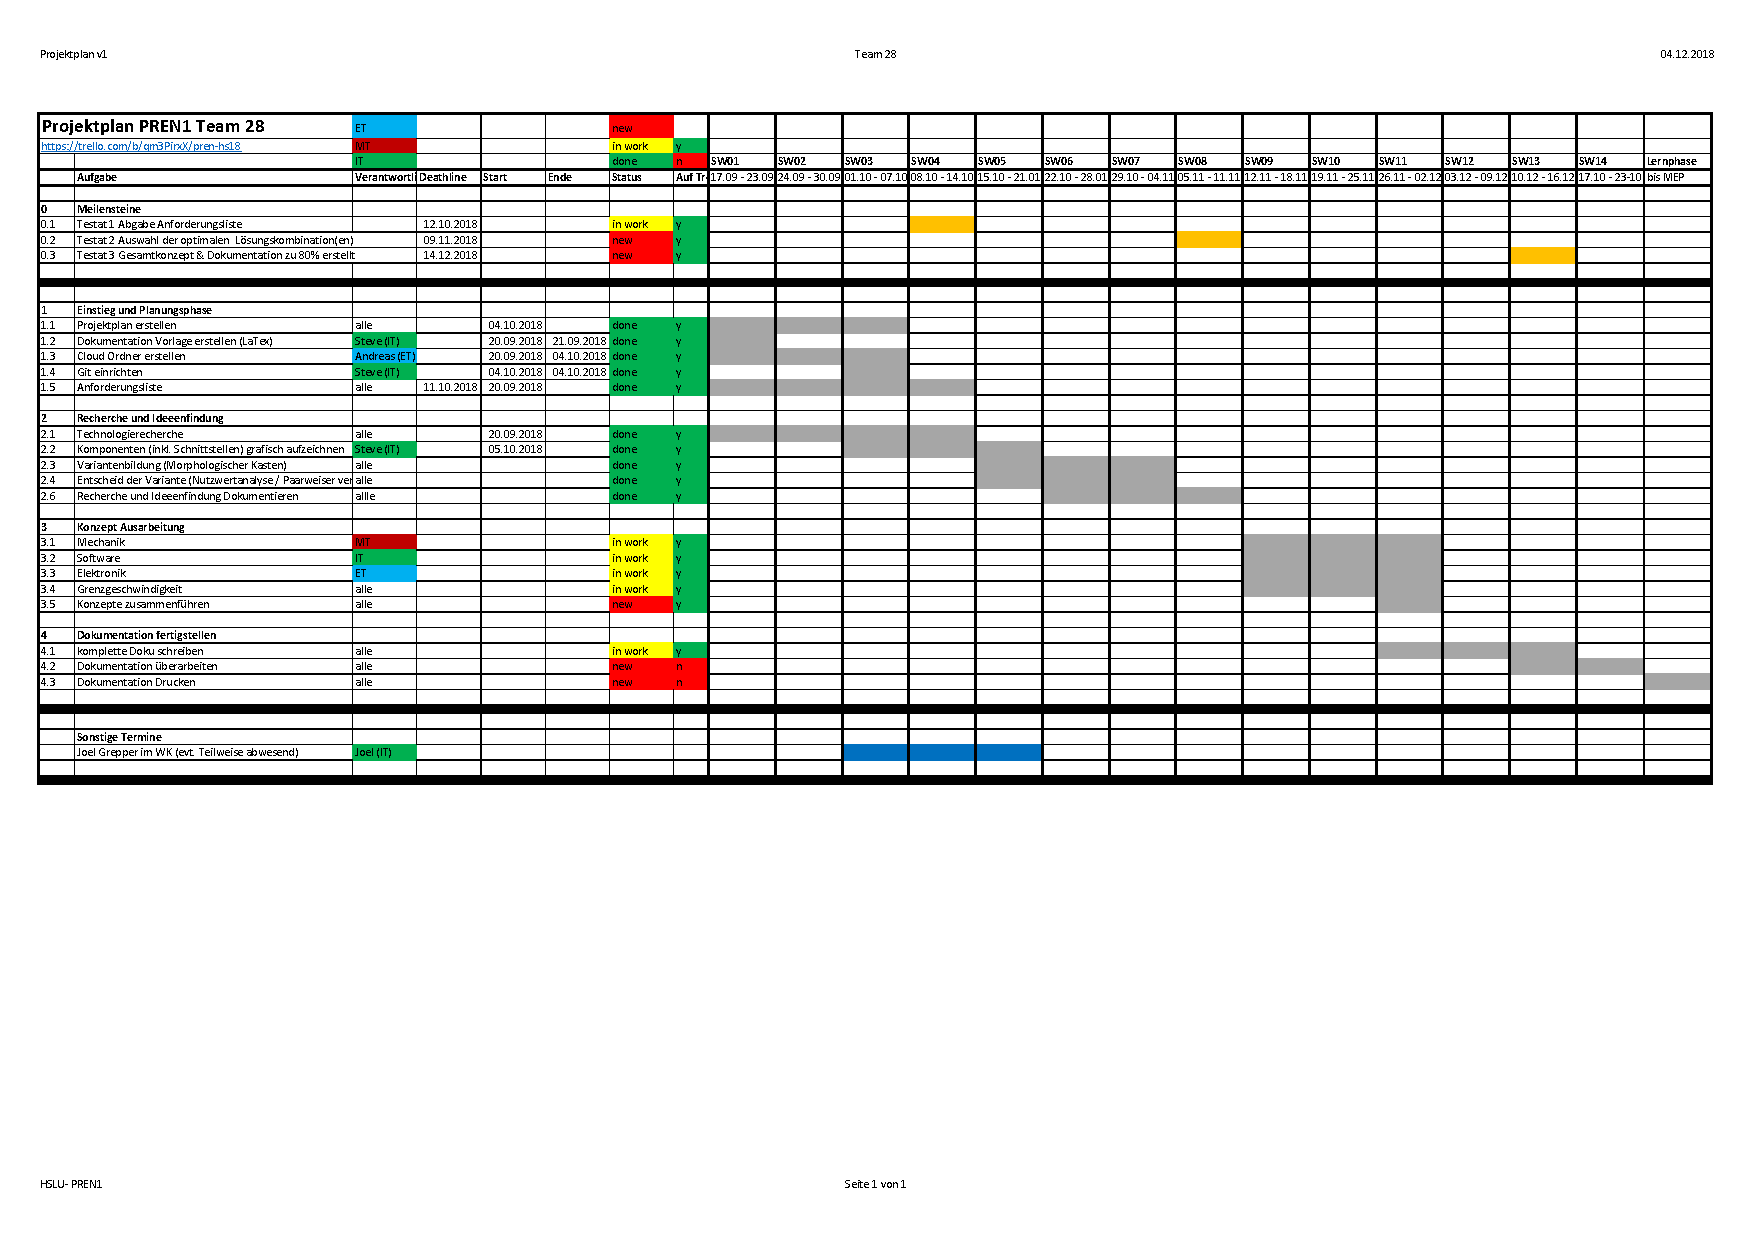
\includegraphics[page=1,width=1\textwidth, trim=.6cm 7cm .6cm 1.5cm, clip]{Projektplanung.pdf}
    \caption{Zeitorientierte Projektstruktur Team 28\\Stand: SW 12}
    \label{fig:projektplanung}
\end{figure}

Die detailliertere Aufteilung dieser Arbeitspakete wird dann in Trello (Abbliding \ref{fig:screenTrello}) vorgenommen. In der Projektstruktur wird lediglich eingetragen, ob ein bestimmtes Arbeitspaket darin in Trello erfasst ist. Dort kann es in mehrere Teilpakete aufgeteilt und bestimmten Personen zugewiesen werden. Die Arbeitspakete in Trello werden je nach Status in die Kategorien ''To do'', ''doing'', oder ''done'' eingeteilt. Separat werden auch noch die Meilensteine festgehalten und als ''done'' gekennzeichnet sobald diese abgeschlossen sind.\\

\begin{figure}[H] \centering
    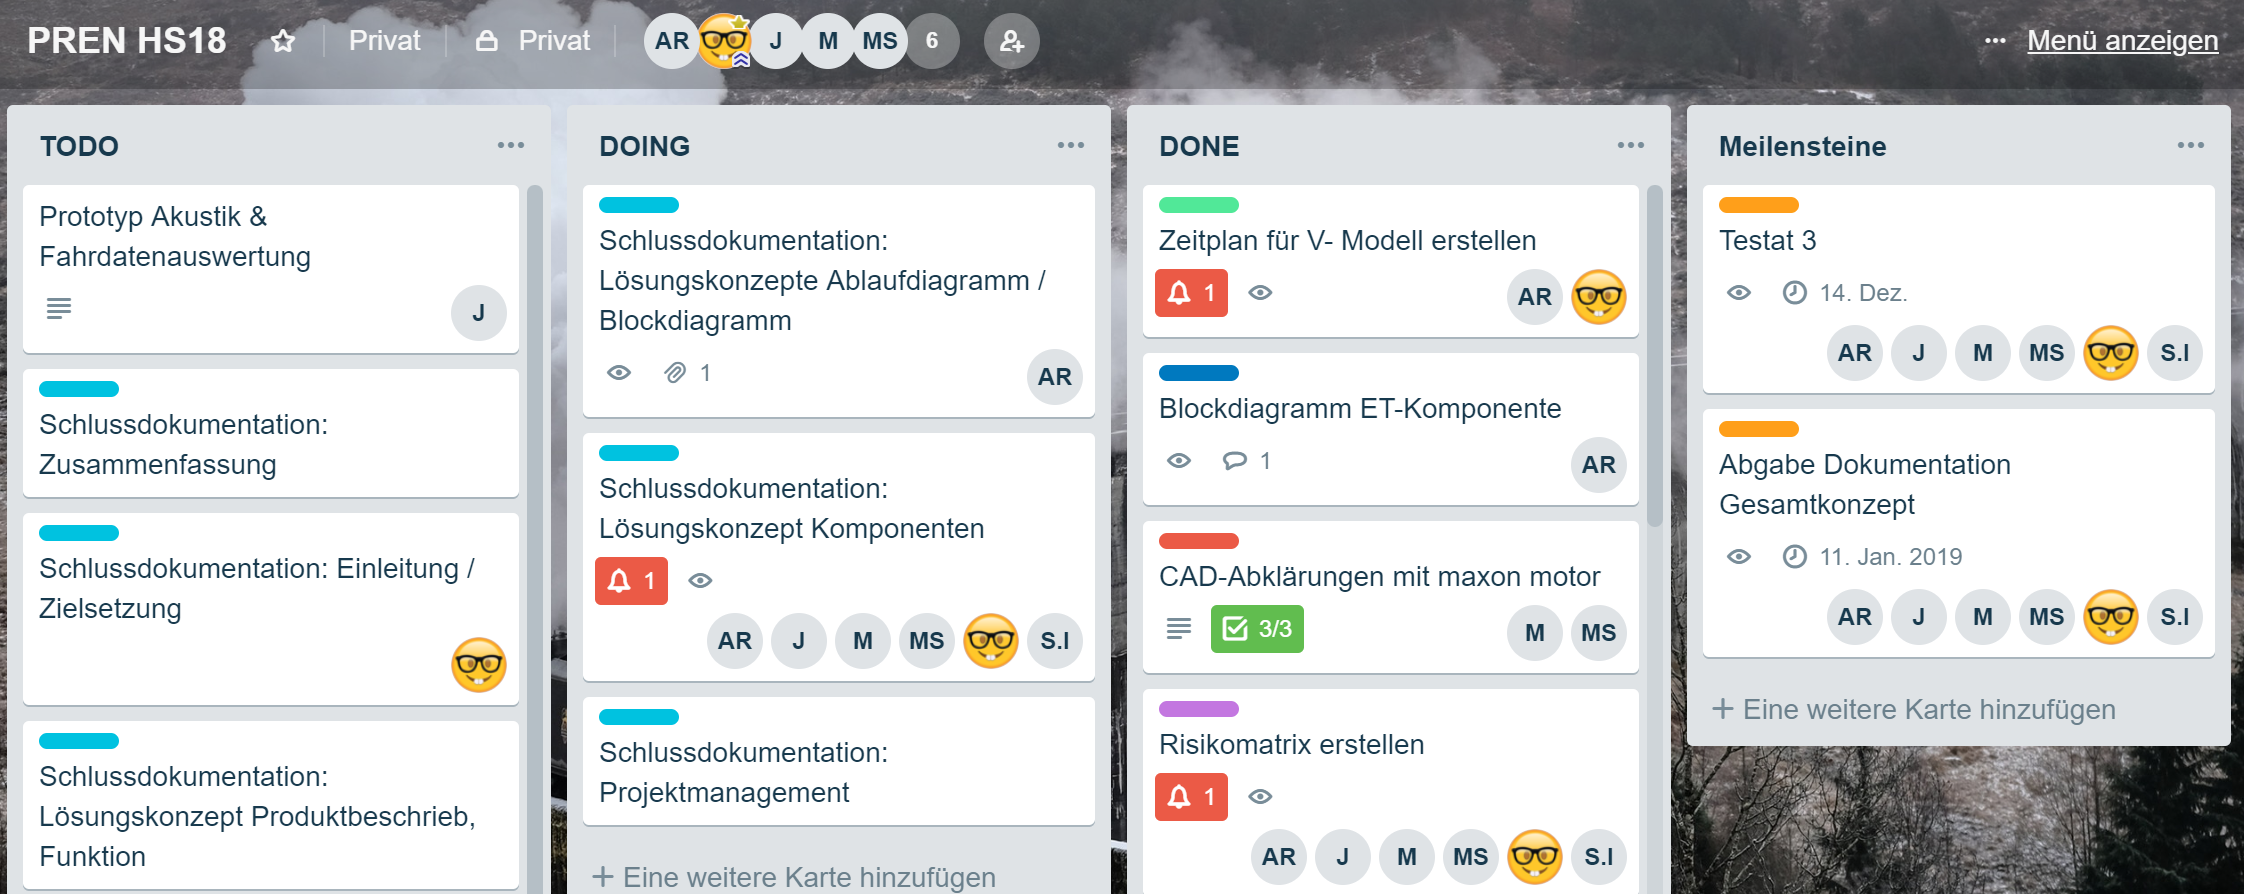
\includegraphics[page=1,width=.8\textwidth]{screenTrello.png}
    \caption{Bildschirmausschnitt Trello Team 28\\Stand: SW 12}
    \label{fig:screenTrello}
\end{figure}
\pagebreak

\subsection{Dokumentation}
Die Dokumentation wird in \LaTeX geschrieben. Der Quell-Text wird in eine normale Text-Datei mit der Endung ".tex" geschrieben. Ein Programm übersetzt diese Quell-Datei dann in ein Dokument wie z.B. ein PDF oder PostScript. \cite{whatislatex}\\
Für die Dokumentation dieses Projekts wird aus dem \LaTeX Code ein PDF erstellt. Der Austausch der Daten im Team erfolgt gemäss Kaptitel \ref{proj_datenaustausch}.

\subsection{Datenaustausch} \label{proj_datenaustausch}
Um Daten im Team auszutauschen, wird auf zwei verschiedene Cloud Plattformen gesetzt. Alle Teammitglieder haben vollständigen Zugriff auf beide Plattformen.\\

\textbf{One Drive}\\
Für diverse Ablagen, Word- und Exceldokumente oder ähnliches steht ein Ordner in Microsoft One Drive zur verfügung. Diese Daten werden jederzeit mit allen Teammitgliedern synchronisiert. In Dokumenten von Microsoft Office ist es auch möglich, dass mehrere Personen zur selben Zeit am selben Dokument arbeiten.\\

\textbf{Github}\\
Es steht ein Github Repository zur Verfügung. Mit dem Programm Git kann man auf die Daten zugreifen und seine Änderungen hochladen. Dabei können alle Änderungen von allen Personen verfolgt werden. Die genaue Verwendung und die benutzten Tools sind für die Teammitglieder direkt im Repository beschrieben.\\
Dieses Repository wird für die Dokumentation und für den Source-Code benutzt. Es gibt einen Ordner für die Dokumentation (alle \LaTeX Dateien, Bilder, Zeichnungen, usw.) und einen weiteren für den Quell-Code. Dort ist der Programmcode für das Raspberry Pi und das Tiny K22 abgelegt.\\
Das Repository kann online unter \url{https://github.com/Inux/pren} eingesehen werden.

\end{document}